% Cover letter: 3D Industrial Designer & CAD Specialist (cycling & sports gear, remote), SUPACAZ
% CV: Sections/cv_industrial_designer_supacaz.tex -> cv_gen/2026-10-27_supacaz/cv_giovanni_tauro-supacaz.pdf
% SUPACAZ only reads LinkedIn DMs: the DM text is in the chat, this letter is for attaching or linking
\documentclass[11pt,a4paper,sans]{moderncv}
% Shared preamble and header for the cover letters.
% One main file per application: cl_<company>.tex, built to
% cv_gen/coverletter_giovanni_tauro-<company>.pdf next to cv_giovanni_tauro-<company>.pdf.
% Paths (cl_gen/..., Pictures/...) are relative to the project root, as in the CV (see .latexmkrc).

\moderncvstyle{classic}
\moderncvcolor{blue}

\usepackage[scale=0.80]{geometry}
\setlength{\footskip}{136.00005pt}

\usepackage{fontawesome5}
% hyperref is loaded by moderncv itself; loading it here causes an option clash
\usepackage{xcolor}
\usepackage{graphicx}
\ifxetexorluatex
  \usepackage{fontspec}
  \usepackage{unicode-math}
  \defaultfontfeatures{Ligatures=TeX}
  \setmainfont{Latin Modern Roman}
  \setsansfont{Latin Modern Sans}
  \setmonofont{Latin Modern Mono}
  \setmathfont{Latin Modern Math}
\else
  \usepackage[T1]{fontenc}
  \usepackage{lmodern}
\fi

\usepackage[english]{babel}

% used for the PDF title and the letter closing; the visible header is \clheader below
\name{Giovanni}{Tauro}

% Header: #1 = headline under the name (same as the headline of the matching CV)
\newcommand{\clheader}[1]{%
\noindent
\begin{minipage}[c]{0.74\textwidth}
    {\Huge \textbf{Giovanni Tauro}}\\[-0.2em]
    {\small #1}\\[0.3em]

    \footnotesize
    \faMapMarker*~
    \href{https://www.google.com/maps/search/?api=1&query=Lecco+23900+Italy}
    {\color{blue}Bari-Lecco, Italy}
    \quad
    \faPhone*~
    \href{https://wa.me/393279437161}
    {\color{blue}+39 3279437161}
    \quad
    \faEnvelope~
    \href{mailto:giovanni.taurodi@gmail.com}
    {\color{blue}giovanni.taurodi@gmail.com}
    \\[-0.1em]

    \faLinkedin~
    \href{https://www.linkedin.com/in/giovanni-tauro-gt/}
    {\color{blue}LinkedIn}
    \quad
    \faGithub~
    \href{https://github.com/jotades}
    {\color{blue}GitHub}
    \quad
    \faGraduationCap~
    \href{https://scholar.google.com/citations?user=BS0aVGgAAAAJ&hl=it}
    {\color{blue}Scholar}
    \quad
    \faFilePdf~
    \href{https://www.notion.so/Giovanni-Tauro-2a7901d92f3a800b892af425c5875c6a}
    {\color{blue}Portfolio}
    \quad
    \faCubes~
    \href{https://grabcad.com/giovanni.tauro-3}
    {\color{blue}GrabCAD}

\end{minipage}
\hfill
\begin{minipage}[c]{0.18\textwidth}
    \raggedleft
    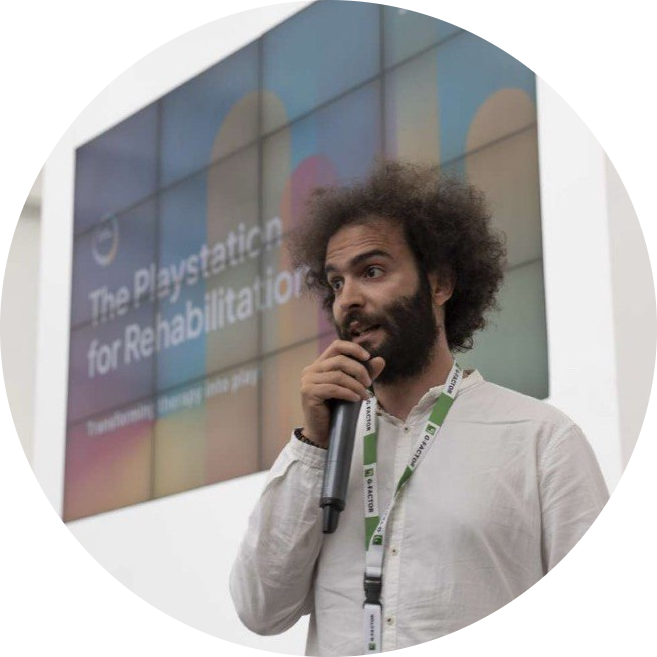
\includegraphics[width=2.8cm]{Pictures/Giovanni_pitch}
\end{minipage}
\vspace{0.1em}
}

\makeatletter
% the sender details are already in \clheader, so skip moderncv's own block
\@detailsfalse
% closing phrase, signature, name
\renewcommand*{\makeletterclosing}{%
  \@closing\\[0.6em]%
  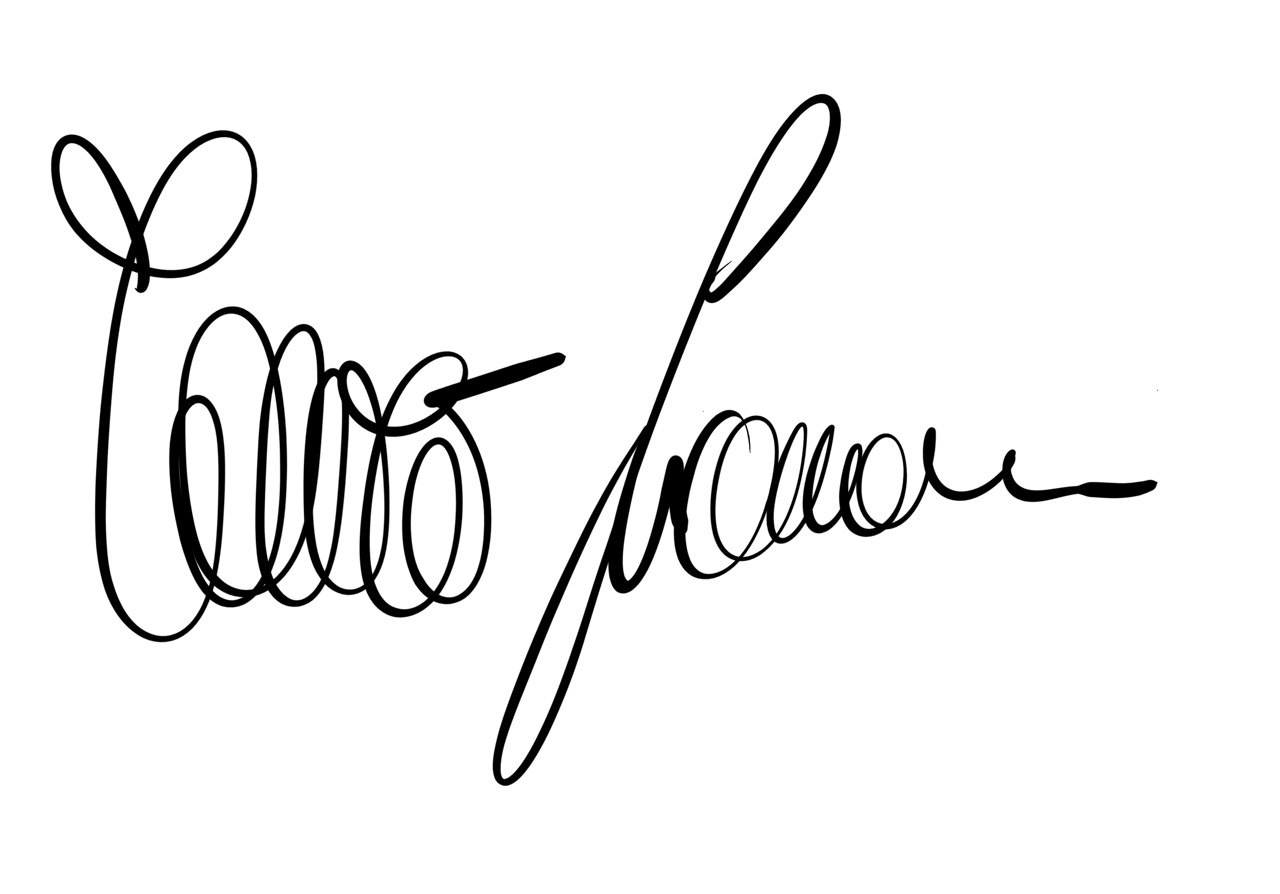
\includegraphics[height=1.2cm]{Pictures/sign_gt.jpg}\\[0.2em]%
  {\bfseries\@firstname~\@lastname}}
\makeatother


\begin{document}

\clheader{Industrial Designer | 3D CAD, Prototyping \& Testing}

\recipient{SUPACAZ}{Remote}
\opening{Dear SUPACAZ Team,}
\closing{Sincerely,}
\makelettertitle

I am applying for the 3D Industrial Designer \& CAD Specialist role. I trained as an industrial designer (BSc, University of Florence; MSc in Design \& Engineering, Politecnico di Milano), and for more than five years I have taken physical products from sketch to tested prototype at CNR-STIIMA, the Italian National Research Council, and as Head of Product and co-founder of Rehabilia Technologies.

My main project is PhiCube, a modular device for neurorehabilitation. I worked on it from user research and concept sketches to mechanical design, assembly and deployment in Italian clinics, and I am a co-inventor on its patent (WO2023214349A1). It reached a usability score of 85.8/100 (SUS) with 19 children and is now in two ongoing multicentre studies with 134 patients. A product that people use with their own bodies, session after session, has to be robust, adjustable and pleasant to use, which is not far from what a rider expects from their gear.

Day to day I model parts, assemblies and technical drawings in SolidWorks and Fusion 360, build prototypes with 3D printing, choose materials and manufacturing methods by batch size, cost and technical constraints, then test and iterate on user feedback and performance data. I document design intent in technical files and manuals, and as Head of Product I coordinate external suppliers and keep engineering, design and clinical partners aligned.

Sport has been part of my design work from the start. As a freelancer with DIMA3D I reverse-engineered parts for extreme-sports, automotive and medtech clients, turning 3D scans into parametric CAD models ready for production. At Adidas, working remotely, I developed sportswear concepts from trend and competitor research, defined materials and colours within the brand's language, and produced Blender renders and an AR experience. Outside work I ride a longboard and hike in the mountains. My research has also taken me to Utrecht and twice to Japan, so working across countries and time zones with California, Taipei and Tokyo would feel familiar.

My products so far have been rehabilitation devices rather than cycling components, and my production experience is mostly 3D printing and small batches: I have not yet taken a carbon-fibre or injection-moulded part to production, and I model in SolidWorks and Fusion 360 rather than Rhino. These are the areas where I would expect to learn the most, working with your engineers and suppliers. My portfolio and GrabCAD models are linked above.

I would welcome the chance to discuss the role further.

\makeletterclosing

\end{document}
